%% This is an example first chapter.  You should put chapter/appendix that you
%% write into a separate file, and add a line \include{yourfilename} to
%% main.tex, where `yourfilename.tex' is the name of the chapter/appendix file.
%% You can process specific files by typing their names in at the 
%% \files=
%% prompt when you run the file main.tex through LaTeX.

\singlespacing{

\chapter{Implementation}

The motivation for this work is to ultimately create a deployable tool that allows others to interact with the virtual environment I've created.  Though it's not central to the themes of this thesis, a lot of time and effort was spent designing an interactive, graphical interface around the ideas discussed in previous chapters. 

\section{Javascript/WebGL}

I used HTML5/Javascript for this application because it allows easier access to the code than any other platform.  Though user studies are not a component of this work, there is a long history of communities of users building things in these types of sandbox environments that surpass anything the developers were able to imagine.  There is a lot of talent beyond the immediate neighborhood of CBA, and I'd like to try to make this codebase as available as possible for anyone interested in exploring this new way of making things.

The app was written with the following dependencies:
\begin{itemize}
\setlength\itemsep{0em}
\item \href{http://threejs.org/}{Three.js} is a library that makes WebGL easy to use without sacrificing much in performance
\item \href{http://requirejs.org/}{RequireJS} is a framework for asynchronously loading javascript modules and dependencies
\item \href{http://backbonejs.org/}{Backbone.js} is a framework for managing UI events and giving structure to an interactive application
\item \href{https://jquery.com/}{JQuery} is a library that simplifies interactions with HTML and helps maintain cross-browser support
\item \href{http://underscorejs.org/}{Underscore} is a library with lots of useful functions for dealing with arrays and javascript objects
\end{itemize}

\section{Performance Speedups}

\subsection{GPU Programming}

\begin{figure}
  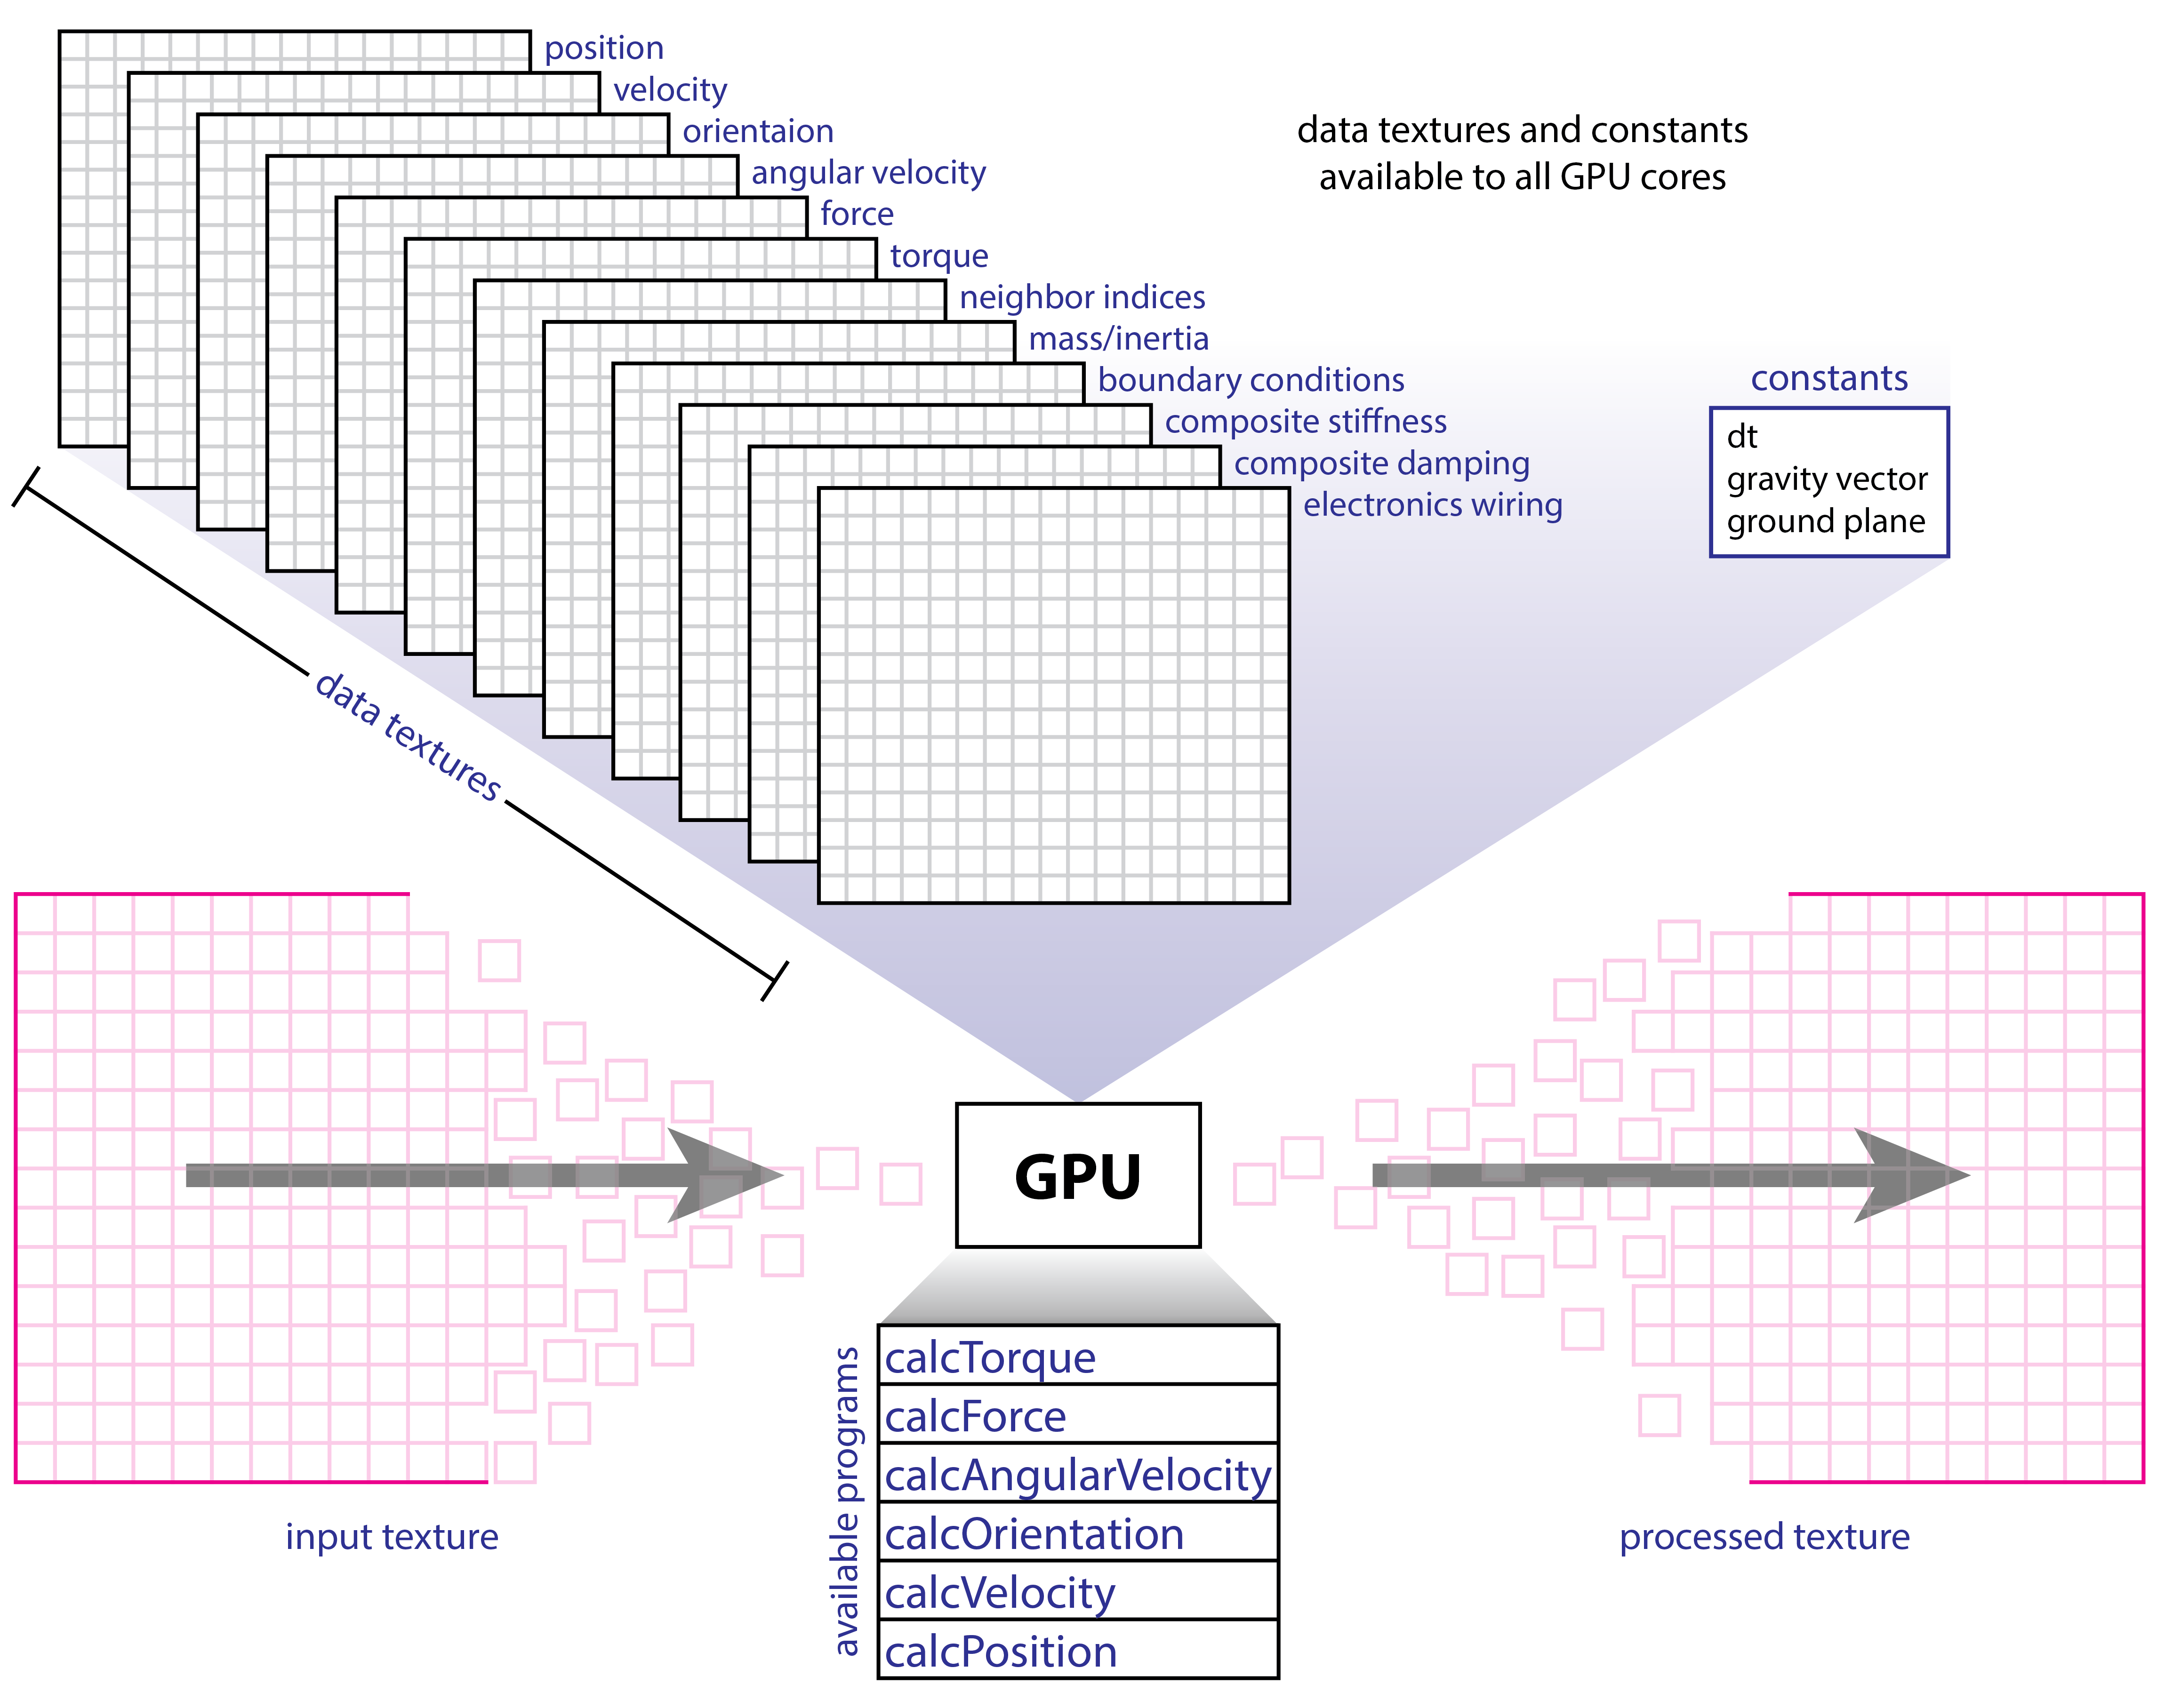
\includegraphics[width=\linewidth]{gpuprogramming.png}
  \caption{.}
  \label{fig:gpuprogramming}
\end{figure}

Computing in the GPU does create some hardware dependencies for this application that would not have otherwise been present.  For example, some GPUs have a hard limit of 8 textures that can be loaded into memory and accessed by each GPU core at a time.  In this case I've implemented a back up \href{https://developer.mozilla.org/en-US/docs/Web/JavaScript/Typed_arrays}{typed array} engine that should be supported by all hardware configurations.


\subsection{Math}

A faster method of applying quaternions to vectors is given by
\[ t = 2 \left[ \begin{array}{ccc}
q_x\\
q_y\\
q_z
 \end{array} \right] \times v\]
\[ v_{rotated} = v + q_wt +  \left[ \begin{array}{ccc}
q_x\\
q_y\\
q_z
 \end{array} \right] \times t\]
 https://blog.molecular-matters.com/2013/05/24/a-faster-quaternion-vector-multiplication/



\section{Numerical Instability}

\begin{figure}
  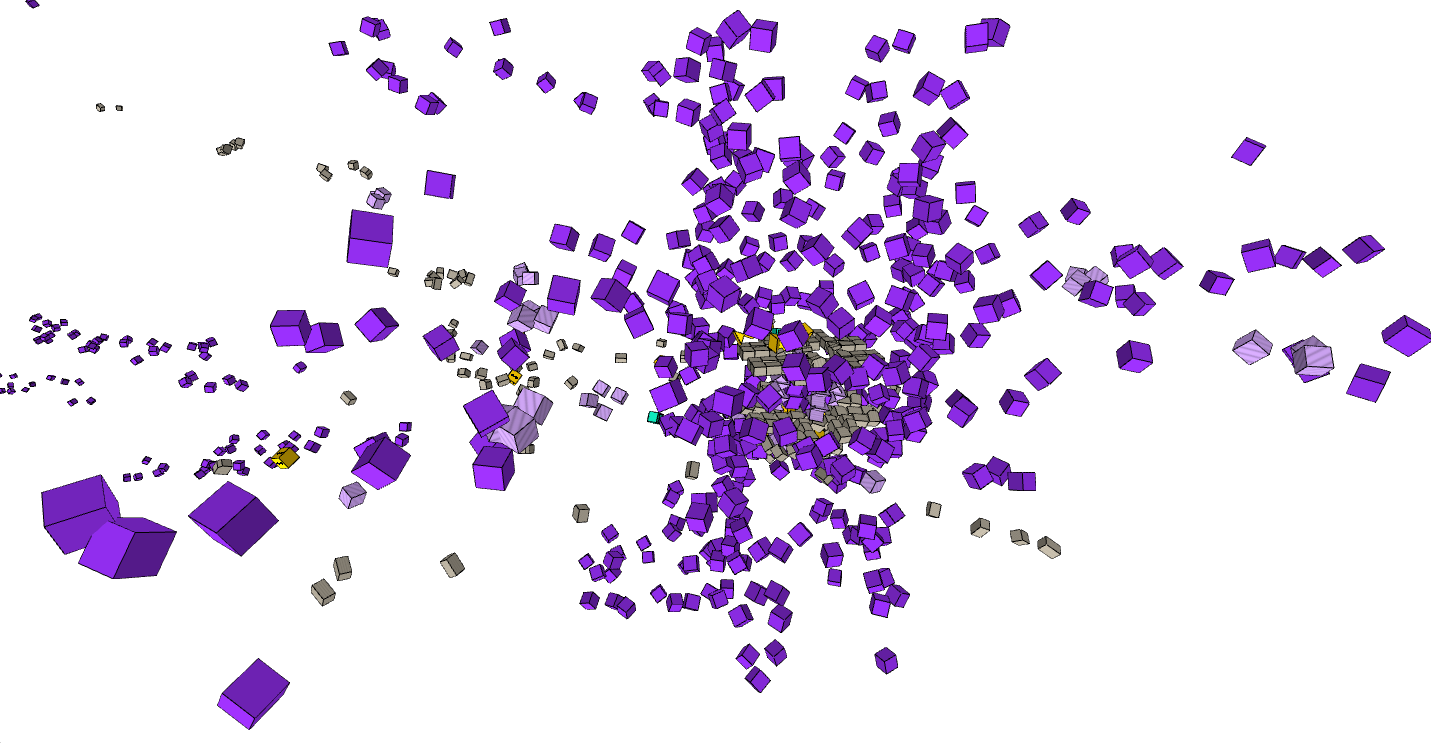
\includegraphics[width=\linewidth]{instability.png}
  \caption{instability.png.}
  \label{fig:instability}
\end{figure}

\section{Examples}
